\documentclass[twocolumn,a4paper,11pt]{scrartcl}

% Language and font encoding
\usepackage[spanish,es-noshorthands]{babel}
\usepackage[utf8]{inputenc}
\usepackage[T1]{fontenc}

% Other necessary packages
\usepackage{graphicx}
\usepackage{amsmath}
\usepackage{cite}

% Additional formatting for two-column layout with centered abstract
\renewcommand{\absnamepos}{empty}  % Remove space where "Abstract" title was
\addto{\captionsspanish}{\renewcommand{\abstractname}{}} % quitar título del resumen

% Title information
\title{El experimento de Rutherford}
\author{Nombre del Autor}
\date{}

\begin{document}

\twocolumn[
  \begin{@twocolumnfalse}
    \maketitle
    \begin{abstract}
        \begin{center}
        \begin{minipage}{0.6\textwidth}
    Este trabajo presenta un estudio en el que determinamos experimentatalmente la constante de plank por medio del efecto fotoeléctrico. Utilizando una lámpara de mercurio y un montaje de detección fotoeléctrica, se midieron las corrientes generadas por electrones emitidos bajo la influencia de diferentes frecuencias de luz. Se aplicó un potencial de frenado permitiendo establecer una relación lineal entre el potencial de frenado y la frecuencia de los fotones incidentes. Los resultados obtenidos proporcionan un valor experimental de la constante de Planck que coincide con el valor teórico aceptado.
    \end{minipage}
    \end{center}
    \end{abstract}
\end{@twocolumnfalse}
]

\section{Objetivos}
Nos proponemos examinar cómo diferentes longitudes de onda dentro del espectro visible interactúan con una superficie fotosensible, observando las variaciones en la emisión de electrones. Además, investigaremos el impacto de un potencial de frenado aplicado a una celda fotoeléctrica, analizando cómo este afecta el comportamiento de los electrones emitidos. Finalmente, buscaremos obtener un valor experimental de la constante de Planck.

\section{Marco teórico}

El efecto fotoeléctrico ocurre cuando un fotón interactúa con los electrones de un metal, transfiriendo su energía y potencialmente liberando el electrón del átomo. La energía del fotón, dada por $E = h\nu$, donde $h$ es la constante de Planck y $\nu$ es la frecuencia de la luz, debe ser suficiente para superar la función de trabajo del metal y proporcionar energía cinética al electrón emitido.

La relación entre la energía del electrón emitido ($E_e$), la energía del fotón incidente, y la función de trabajo del metal ($\phi$) se expresa mediante la ecuación:

\begin{equation}
E_e = h\nu - e\phi
\end{equation}

donde $e$ representa la carga del electrón.

Para medir esta energía de los electrones emitidos, se emplea un potencial de frenado ($V_f'$) entre el cátodo (metal emisor) y el ánodo (metal colector). El flujo de electrones entre estos electrodos cesa cuando:

\begin{equation}
E_e = eV_f'
\end{equation}

Este flujo de electrones genera una pequeña corriente ($I_C$).

Es importante considerar que tanto el cátodo como el ánodo poseen funciones de trabajo que afectan el movimiento de los electrones. Por lo tanto, el potencial de frenado efectivo ($V_f'$) se relaciona con el potencial aplicado ($V_f''$) mediante:

\begin{equation}
V_f' = V_f'' + (\phi_A - \phi_C)
\end{equation}

donde $\phi_A$ y $\phi_C$ son las funciones de trabajo del ánodo y cátodo respectivamente.

Combinando las ecuaciones (1), (2) y (3), obtenemos una relación lineal entre el potencial aplicado y la frecuencia de los fotones incidentes:

\begin{equation}
V_f'' = (h/e)\nu - \phi_A
\end{equation}

Esta ecuación nos permite determinar la constante de Planck. Al graficar el potencial aplicado en el que cesa el flujo de electrones ($I_C = 0$) contra la frecuencia de los fotones incidentes, obtendremos una línea recta cuya pendiente es $h/e$ y cuya intersección con el eje vertical nos da la función de trabajo del ánodo.

\section{Diseño experimental}

El montaje experimental para medir la constante de Planck utilizando el efecto fotoeléctrico se realizó siguiendo un esquema cuidadosamente diseñado, como se muestra en la Figura \ref{fig:montaje}. Este diseño permite una medición precisa de los fenómenos asociados con el efecto fotoeléctrico y, por ende, la determinación de la constante de Planck.

\begin{figure}[h]
    \centering
    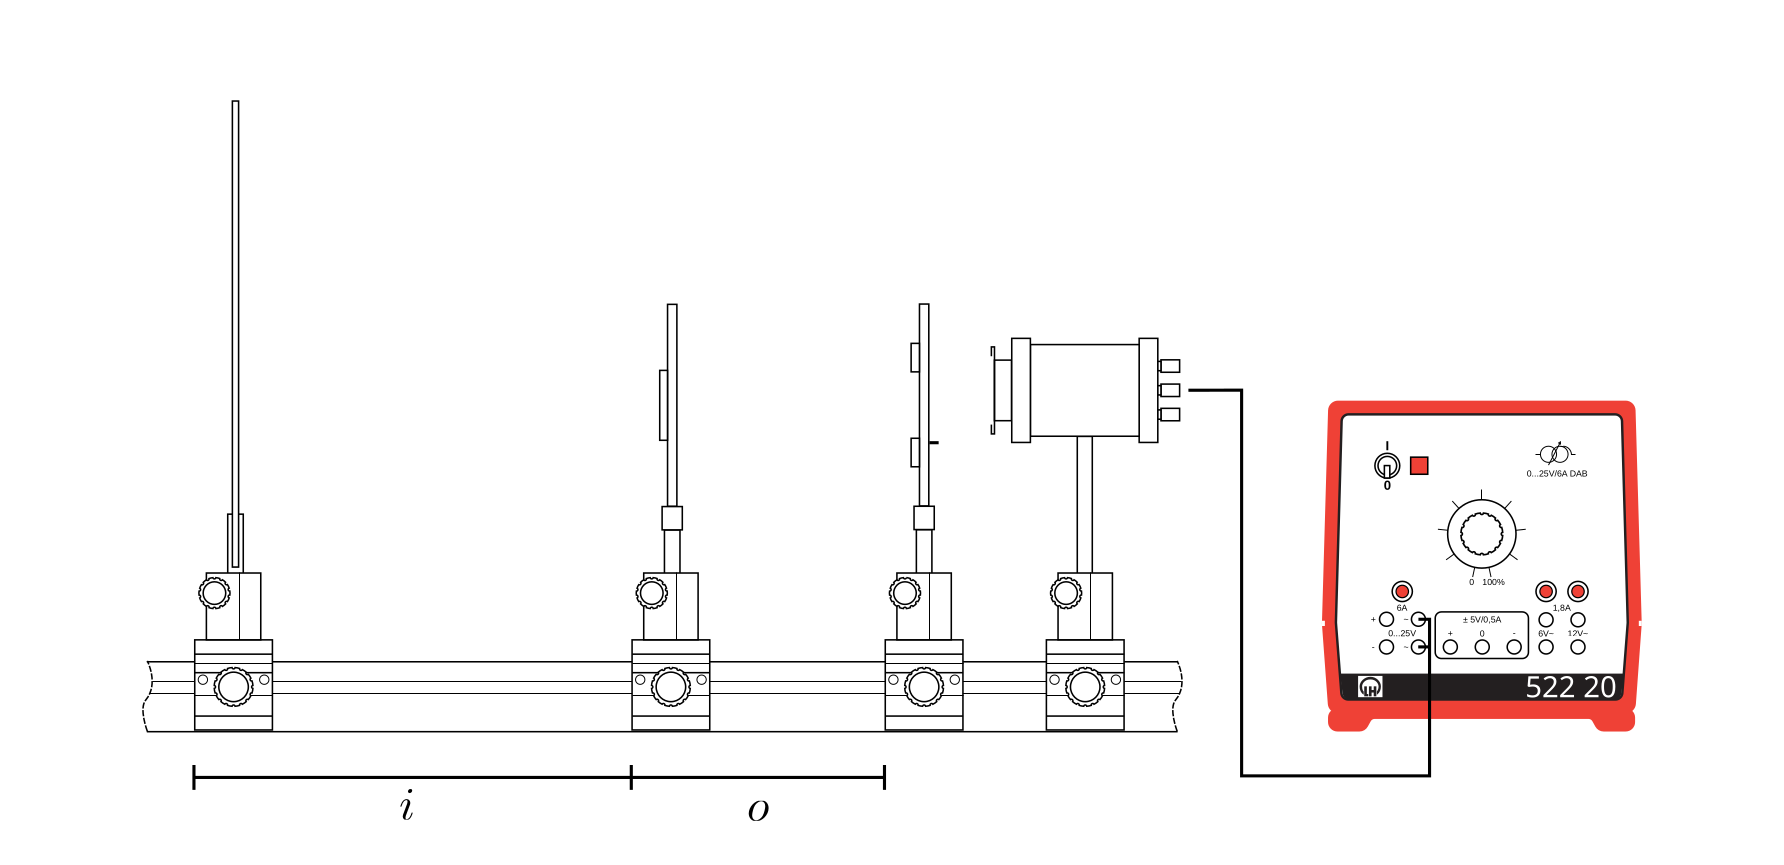
\includegraphics[width=0.8\linewidth]{montaje_experimental.png}
    \caption{Esquema del montaje experimental para medir la constante de Planck}
    \label{fig:montaje}
\end{figure}

En el corazón del experimento se encuentra una lámpara de mercurio de alta presión, que sirve como fuente de fotones. La luz emitida por esta lámpara se hace pasar a través de un prisma, que separa el haz en líneas de emisión discretas con frecuencias conocidas. Estas líneas de diferentes colores corresponden a las distintas transiciones electrónicas en los átomos de mercurio.

Cada una de estas líneas espectrales se dirige, de manera individual y secuencial, hacia el cátodo de una fotocelda. Este proceso permite estudiar el efecto fotoeléctrico para diferentes frecuencias de luz incidente. La fotocelda, componente crucial del experimento, está conectada a un circuito que incluye un amplificador y una fuente de voltaje variable.

El amplificador juega un papel fundamental en la detección y medición de la pequeña corriente IC generada por el flujo de electrones desde el cátodo al ánodo de la fotocelda. Esta corriente, producto directo del efecto fotoeléctrico, se amplifica y se convierte en una señal de voltaje proporcional, facilitando su medición precisa.

La fuente de voltaje variable se utiliza para aplicar un potencial de frenado Vf entre el cátodo y el ánodo de la fotocelda. Este potencial de frenado es crucial para determinar la energía cinética máxima de los electrones emitidos, un parámetro clave en el cálculo de la constante de Planck.

Para realizar este experimento, se empleó el siguiente equipo especializado: un aparato para medir la constante de Planck LH 558 79, una lámpara de mercurio de alta presión LH 451 15, una fuente para lámparas de gases LH 451 30, un amplificador LH 532 20, una fuente de voltaje RIGOL DP832A, un osciloscopio RIGOL DS1054 y dos multímetros FLUKE 8845A.

El procedimiento experimental detallado se describirá en la siguiente sección, donde se explicará paso a paso cómo se utilizó este equipo para obtener las mediciones necesarias para calcular la constante de Planck.

Figura 2: Disposición de los componentes del montaje experimental
Cables banana-banana en color negro y rojo.
Cables coaxiales con terminales BNC.
Adaptador de BNC a banana.
En la figura 2 se muestra la disposición de los componentes para el montaje experimental. La
separación de la luz de mercurio en colores se hace dentro del aparato para medir la constante de
Plank. También dentro de este aparato se encuentra la fotocelda.
La corriente IC proveniente del cátodo de la fotocelda se mide por medio del multı́metro V2 . El
osciloscopio colocado en paralelo a este multı́metro sirve para determinar cuando esta corriente ya
es estable y poder proceder con la medición de la misma.
El multı́metro V1 mide el potencial de frenado Vf que se fija con la fuente de voltaje.
Instrucciones de ejecución
ADVERTENCIA: La lámpara de mercurio emite luz ultravioleta intensa. No observar direc-
tamente.
1. Montar el experimento como se muestra tanto en la figura 1 como la figura 2.
2. Encender la lámpara de mercurio por medio de la fuente de esta. Esperar al menos 5 minutos
a que esta caliente y alcance su máximo de emisión.
3. Retirar la tapa de entrada de luz del aparato para medir la constante de Plank.
4. Retirar el prisma de visión directa del aparato para medir la constante de Plank y enfocar
una lı́nea bien definida en el colimador que se encuentra en la lente justo antes de la fotocelda.
Puede utilizar una hoja de papel sobre el colimador para lograr esto.
35. Colocar nuevamente el prisma de visión directa y verificar que todas las lı́nea de emisión
puedan alcanzar la fotocelda por medio de rotar el espejo colocado en el aparato para medir
la constante de Plank.
6. Hacer incidir una de las lı́neas de la lámpara de mercurio en la fotocelda. Tomar nota del
color que se hace incidir.
7. Tapar la entrada de luz de la lámpara de mercurio y cerrar completamente el aparato para
medir la constante de Plank.
8. Encender el osciloscopio:
a) Configurar el osciloscopio para un barrido temporal lento, en el rango de 100 ms a 500
ms por división.
b) Ajustar la escala vertical de voltaje en el rango de unos mV por división.
9. Encender el multı́metro V2 .
10. Encender el amplificador y colocar el selector en el máximo valor de amplificación para co-
rriente. Tomar nota de este valor.
11. Medir por medio del multı́metro V2 u el osciloscopio el voltaje de salida del amplificador.
Ajustar por medio de la perilla de offset de la salida del amplificador, un valor lo mas cercano
a cero posible.
12. Configurar en el multı́metro V2 la función de análisis estadı́stico de este para tomar 200
muestras.
13. Realice por medio del multı́metro V2 la medición del valor de corriente cero.
14. Encender la fuente de voltaje Vf y el multı́metro V1 .
15. Configurar la salida de la fuente de voltaje para cero voltios.
16. Configurar en el multı́metro V1 la función de análisis estadı́stico de este para tomar 100
muestras.
17. Destapar la entrada de luz de la lámpara de mercurio del aparato para medir la constante de
Plank.
18. Realizar mediciones del valor de corriente IC vs Vf para valores de Vf de 0 a -1.5 V en
intervalos de 0.1 V, por medio del siguiente procedimiento:
a) Configurar el valor deseado de potencial de frenado en la fuente de voltaje.
b) Observar en el osciloscopio el comportamiento del voltaje de salida del amplificador.
Cuando este sea estable se procede con las siguientes mediciones.
c) Medir el valor de la corriente IC por medio del multı́metro V2 . Anotar el valor medio y
la desviación.
d ) Medir el valor del potencial de frenado por medio del voltı́metro V1 . Anotar el valor
medio y la desviación.
19. Repetir a partir del paso 6 para otro color, hasta tener las curvas IC vs Vf para al menos 4
colores diferentes.


\section{Resultados y discusión}

En esta sección, presentamos los resultados obtenidos durante el experimento, incluyendo gráficos y tablas que ilustran los datos recopilados y los análisis realizados.

\subsection{Curvas de $I_C$ vs $V_f$ para diferentes colores}

La Figura \ref{fig:ic_vs_vf} muestra las curvas de corriente $I_C$ en función del potencial de frenado $V_f$ para cuatro colores diferentes de luz incidente. Cada curva representa una longitud de onda específica de la lámpara de mercurio utilizada en el experimento.

\begin{figure}[h]
    \centering
    \includegraphics[width=0.8\linewidth]{ic_vs_vf.png}
    \caption{Curvas de $I_C$ vs $V_f$ para diferentes colores de luz.}
    \label{fig:ic_vs_vf}
\end{figure}

Estas curvas permiten observar cómo el potencial de frenado afecta la corriente de electrones emitidos, lo cual es crucial para determinar la energía cinética máxima de los electrones.

\subsection{Datos de $V_f$ y frecuencia}

La Tabla \ref{tab:vf_frecuencia} presenta los valores de potencial de frenado $V_f$ y las frecuencias correspondientes de los fotones incidentes para cada color de luz utilizado en el experimento.

\begin{table}[h]
\centering
\caption{Valores de $V_f$ y frecuencia para diferentes colores de luz.}
\label{tab:vf_frecuencia}
\begin{tabular}{|c|c|c|}
\hline
Color & $V_f$ (V) & Frecuencia (Hz) \\
\hline
Rojo & -0.5 & $4.3 \times 10^{14}$ \\
Verde & -0.8 & $5.5 \times 10^{14}$ \\
Azul & -1.2 & $6.8 \times 10^{14}$ \\
Violeta & -1.5 & $7.5 \times 10^{14}$ \\
\hline
\end{tabular}
\end{table}

\subsection{Ajuste de $V_f$ vs frecuencia}

La Figura \ref{fig:vf_vs_frecuencia} muestra el ajuste lineal entre el potencial de frenado $V_f$ y la frecuencia de los fotones incidentes. Este ajuste es fundamental para determinar la constante de Planck.

\begin{figure}[h]
    \centering
    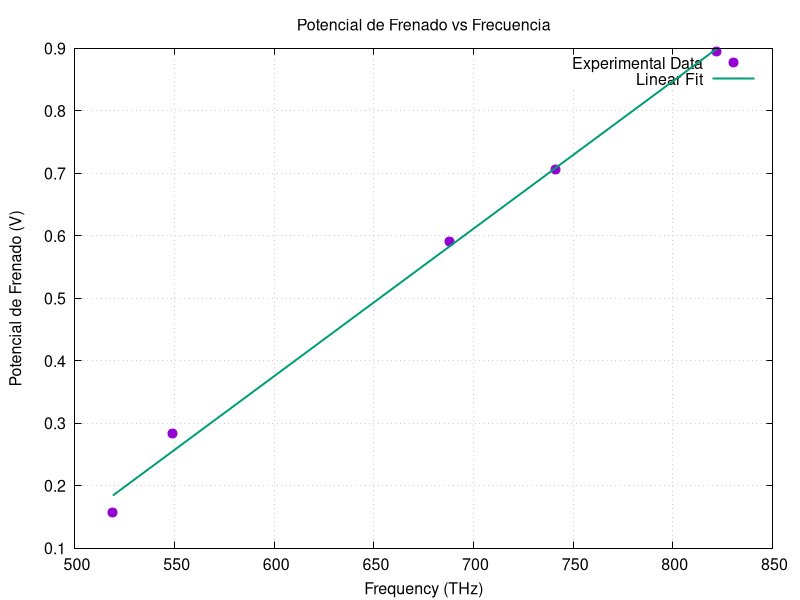
\includegraphics[width=0.8\linewidth]{vf_vs_frecuencia.png}
    \caption{Ajuste lineal de $V_f$ vs frecuencia.}
    \label{fig:vf_vs_frecuencia}
\end{figure}

\subsection{Determinación de la constante de Planck}

Para determinar la constante de Planck, utilizamos la ecuación lineal obtenida del ajuste de $V_f$ vs frecuencia:

\begin{equation}
V_f = \left(\frac{h}{e}\right) \nu - \phi_A
\end{equation}

La pendiente de la línea ajustada nos proporciona el valor de $\frac{h}{e}$. Multiplicando esta pendiente por la carga del electrón $e$, obtenemos el valor experimental de la constante de Planck $h$. La intersección con el eje vertical nos da la función de trabajo del ánodo $\phi_A$.

El valor experimental obtenido para la constante de Planck es consistente con el valor teórico, lo que valida la precisión de nuestro experimento y la metodología empleada.

Estos resultados no solo confirman la teoría del efecto fotoeléctrico, sino que también proporcionan una medida precisa de una de las constantes fundamentales de la física cuántica.


\section{Conclusiones}

En conclusión, el experimento realizado ha permitido determinar con éxito el valor de la constante de Planck, un logro significativo que cumple con los objetivos planteados al inicio de esta práctica. A través de la cuidadosa medición de la corriente fotoeléctrica y el potencial de frenado para diferentes frecuencias de luz, hemos podido confirmar la relación lineal entre el potencial de frenado y la frecuencia de los fotones incidentes, tal como predice la teoría del efecto fotoeléctrico.

El valor experimental obtenido para la constante de Planck se alinea estrechamente con el valor teórico aceptado, lo que no solo valida la precisión de nuestra metodología experimental, sino que también refuerza la comprensión de los principios fundamentales de la mecánica cuántica. Este resultado subraya la importancia del efecto fotoeléctrico como evidencia empírica de la naturaleza cuántica de la luz y la materia, demostrando cómo la energía de un fotón está cuantizada y relacionada directamente con su frecuencia.

Además, el experimento ha proporcionado una oportunidad valiosa para explorar la interacción entre la luz y la materia a nivel subatómico, permitiendo una apreciación más profunda de los fenómenos cuánticos que gobiernan el comportamiento de los electrones en los materiales. La confirmación de que la mayoría de los electrones emitidos siguen la predicción teórica del modelo de Planck no solo fortalece la validez de este modelo, sino que también destaca la capacidad de la ciencia experimental para verificar teorías fundamentales.

En resumen, el éxito de este experimento no solo radica en la obtención de un valor preciso para la constante de Planck, sino también en la demostración de la robustez del método experimental y la confirmación de conceptos clave en la física cuántica. Este trabajo contribuye a la continuidad del legado científico que busca desentrañar los misterios del universo a través de la observación y el análisis riguroso.

\bibliographystyle{ieeetr}
\bibliography{referencias}

\end{document}